% LTeX: language=de-DE

\documentclass{article}
\usepackage{listings}
\usepackage{xcolor}
\usepackage{graphicx}
\usepackage[ngerman]{babel}
\usepackage{float}

\definecolor{codegreen}{rgb}{0,0.6,0}
\definecolor{codegray}{rgb}{0.5,0.5,0.5}
\definecolor{codepurple}{rgb}{0.58,0,0.82}
\definecolor{backcolour}{rgb}{0.95,0.95,0.92}

\lstdefinestyle{mystyle}{
    backgroundcolor=\color{backcolour},   
    commentstyle=\color{codegreen},
    keywordstyle=\color{magenta},
    numberstyle=\tiny\color{codegray},
    stringstyle=\color{codepurple},
    basicstyle=\ttfamily\footnotesize,
    breakatwhitespace=false,         
    breaklines=true,                 
    captionpos=b,                    
    keepspaces=true,                 
    numbers=left,                    
    numbersep=5pt,                  
    showspaces=false,                
    showstringspaces=false,
    showtabs=false,                  
    tabsize=2
}

\lstset{style=mystyle}

\begin{document}
    Zu Beginn wird das Schieberegister zurückgesetzt.
    Danach werden die einzelnen Bits der Zahl 21 mit jedem Takt an das Schieberegister übertragen.
    Dabei ist darauf zu achten, dass die Zeit zwischen den Signalwechsel lang genug ist. \\

    \lstinputlisting[language=c++]{../shift_register.ino}

    \begin{figure}[h]
        \centering
        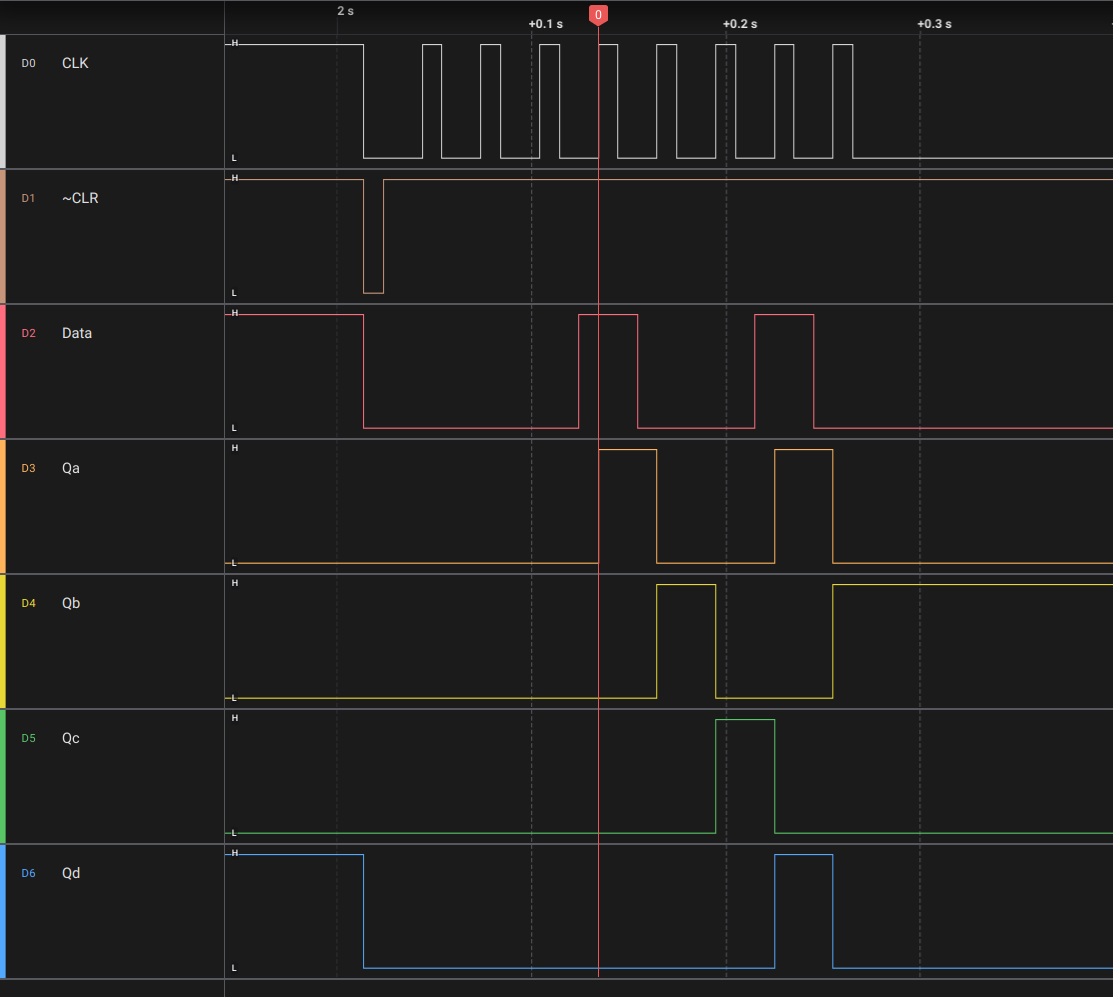
\includegraphics[width=\linewidth]{../measurement1.png}
        \caption{Messung von Qa bis Qd}
    \end{figure}

    \begin{figure}
        \centering
        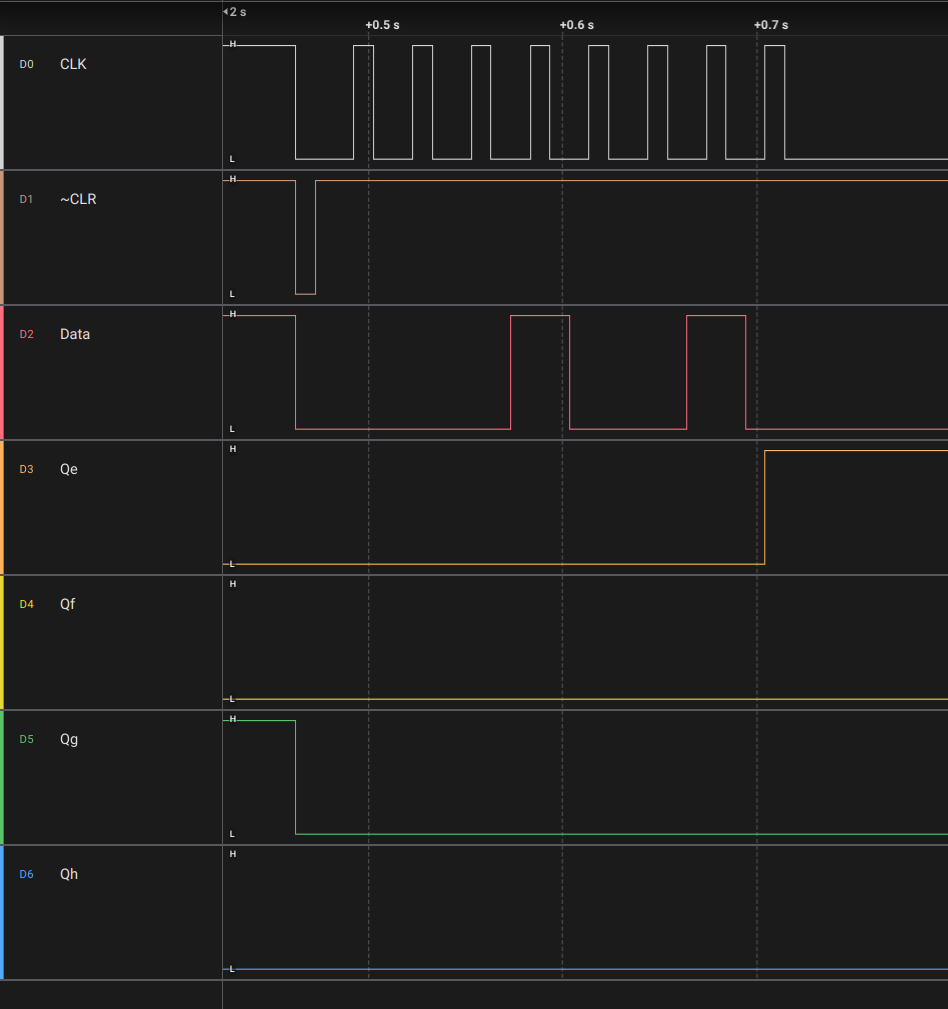
\includegraphics[width=\linewidth]{../measurement2.png}
        \caption{Messung von Qe bis Qh}
    \end{figure}
\end{document}
